\documentclass{report}
\usepackage{graphicx}

\begin{document}

\title{Calculating the work function of a metallic surface with ABINIT}

\author{Matthieu Verstraete, Univeristy of Li\`ege, Belgium}

\maketitle
Copyright (C) 2014-2020 ABINIT group (MV)

This file is distributed under the terms of the
GNU General Public License, see ~abinit/COPYING
or http://www.gnu.org/copyleft/gpl.txt.
For the initials of contributors, see ~abinit/doc/developers/contributors.txt

This brief tutorial should teach you how to calculate a work function $\phi$ for a (metallic) surface, using the ABINIT code. We will presume you know how to calculate a ground state, and have done the first 4 tutorials of ABINIT.

The experimental work function of the Gold (111) surface is 5.2 eV (habitual for metal surfaces which are between 3.5 and 7 eV habitually), and corresponds to the minimal energy required to extract an electron from the surface and bring it to a detector, which is a macroscopic distance away in the vacuum above the surface. The work function in DFT is estimated as the difference between $V(\infty)$, the value of the electronic potential in the vacuum, and the Fermi level $E_F$, which is the energy of the highest lying electron, which is the easiest to extract. The electron density at the surface will spill out some and re-arrange self-consistently when we obtain the ground state. The resulting surface dipole determines the potential step which is experienced between the center of the slab and the vacuum region.

\section{Slab calculation}
We will now perform a straight slab calculation. All of this is severely unconverged in number of k-points, kinetic energy cutoff,  slab thickness and vacuum thicknesses. The input file i.au describes a slab of 3 layers of gold, stacked along the (111) direction (ABC stacking). The full height of the supercell is 10 times the inter-layer distance, such that the fractional coordinates of the layers are easy to calculate, and there are 10-3=7 ``layers'' of vacuum (which corresponds to 21 Angstrom). Another thing we will not converge is the atomic positions: there should be some relaxation of the interlayer distances at the surface, and you should do a structural relaxation to get an accurate result.

\begin{figure}[h]
\begin{center}
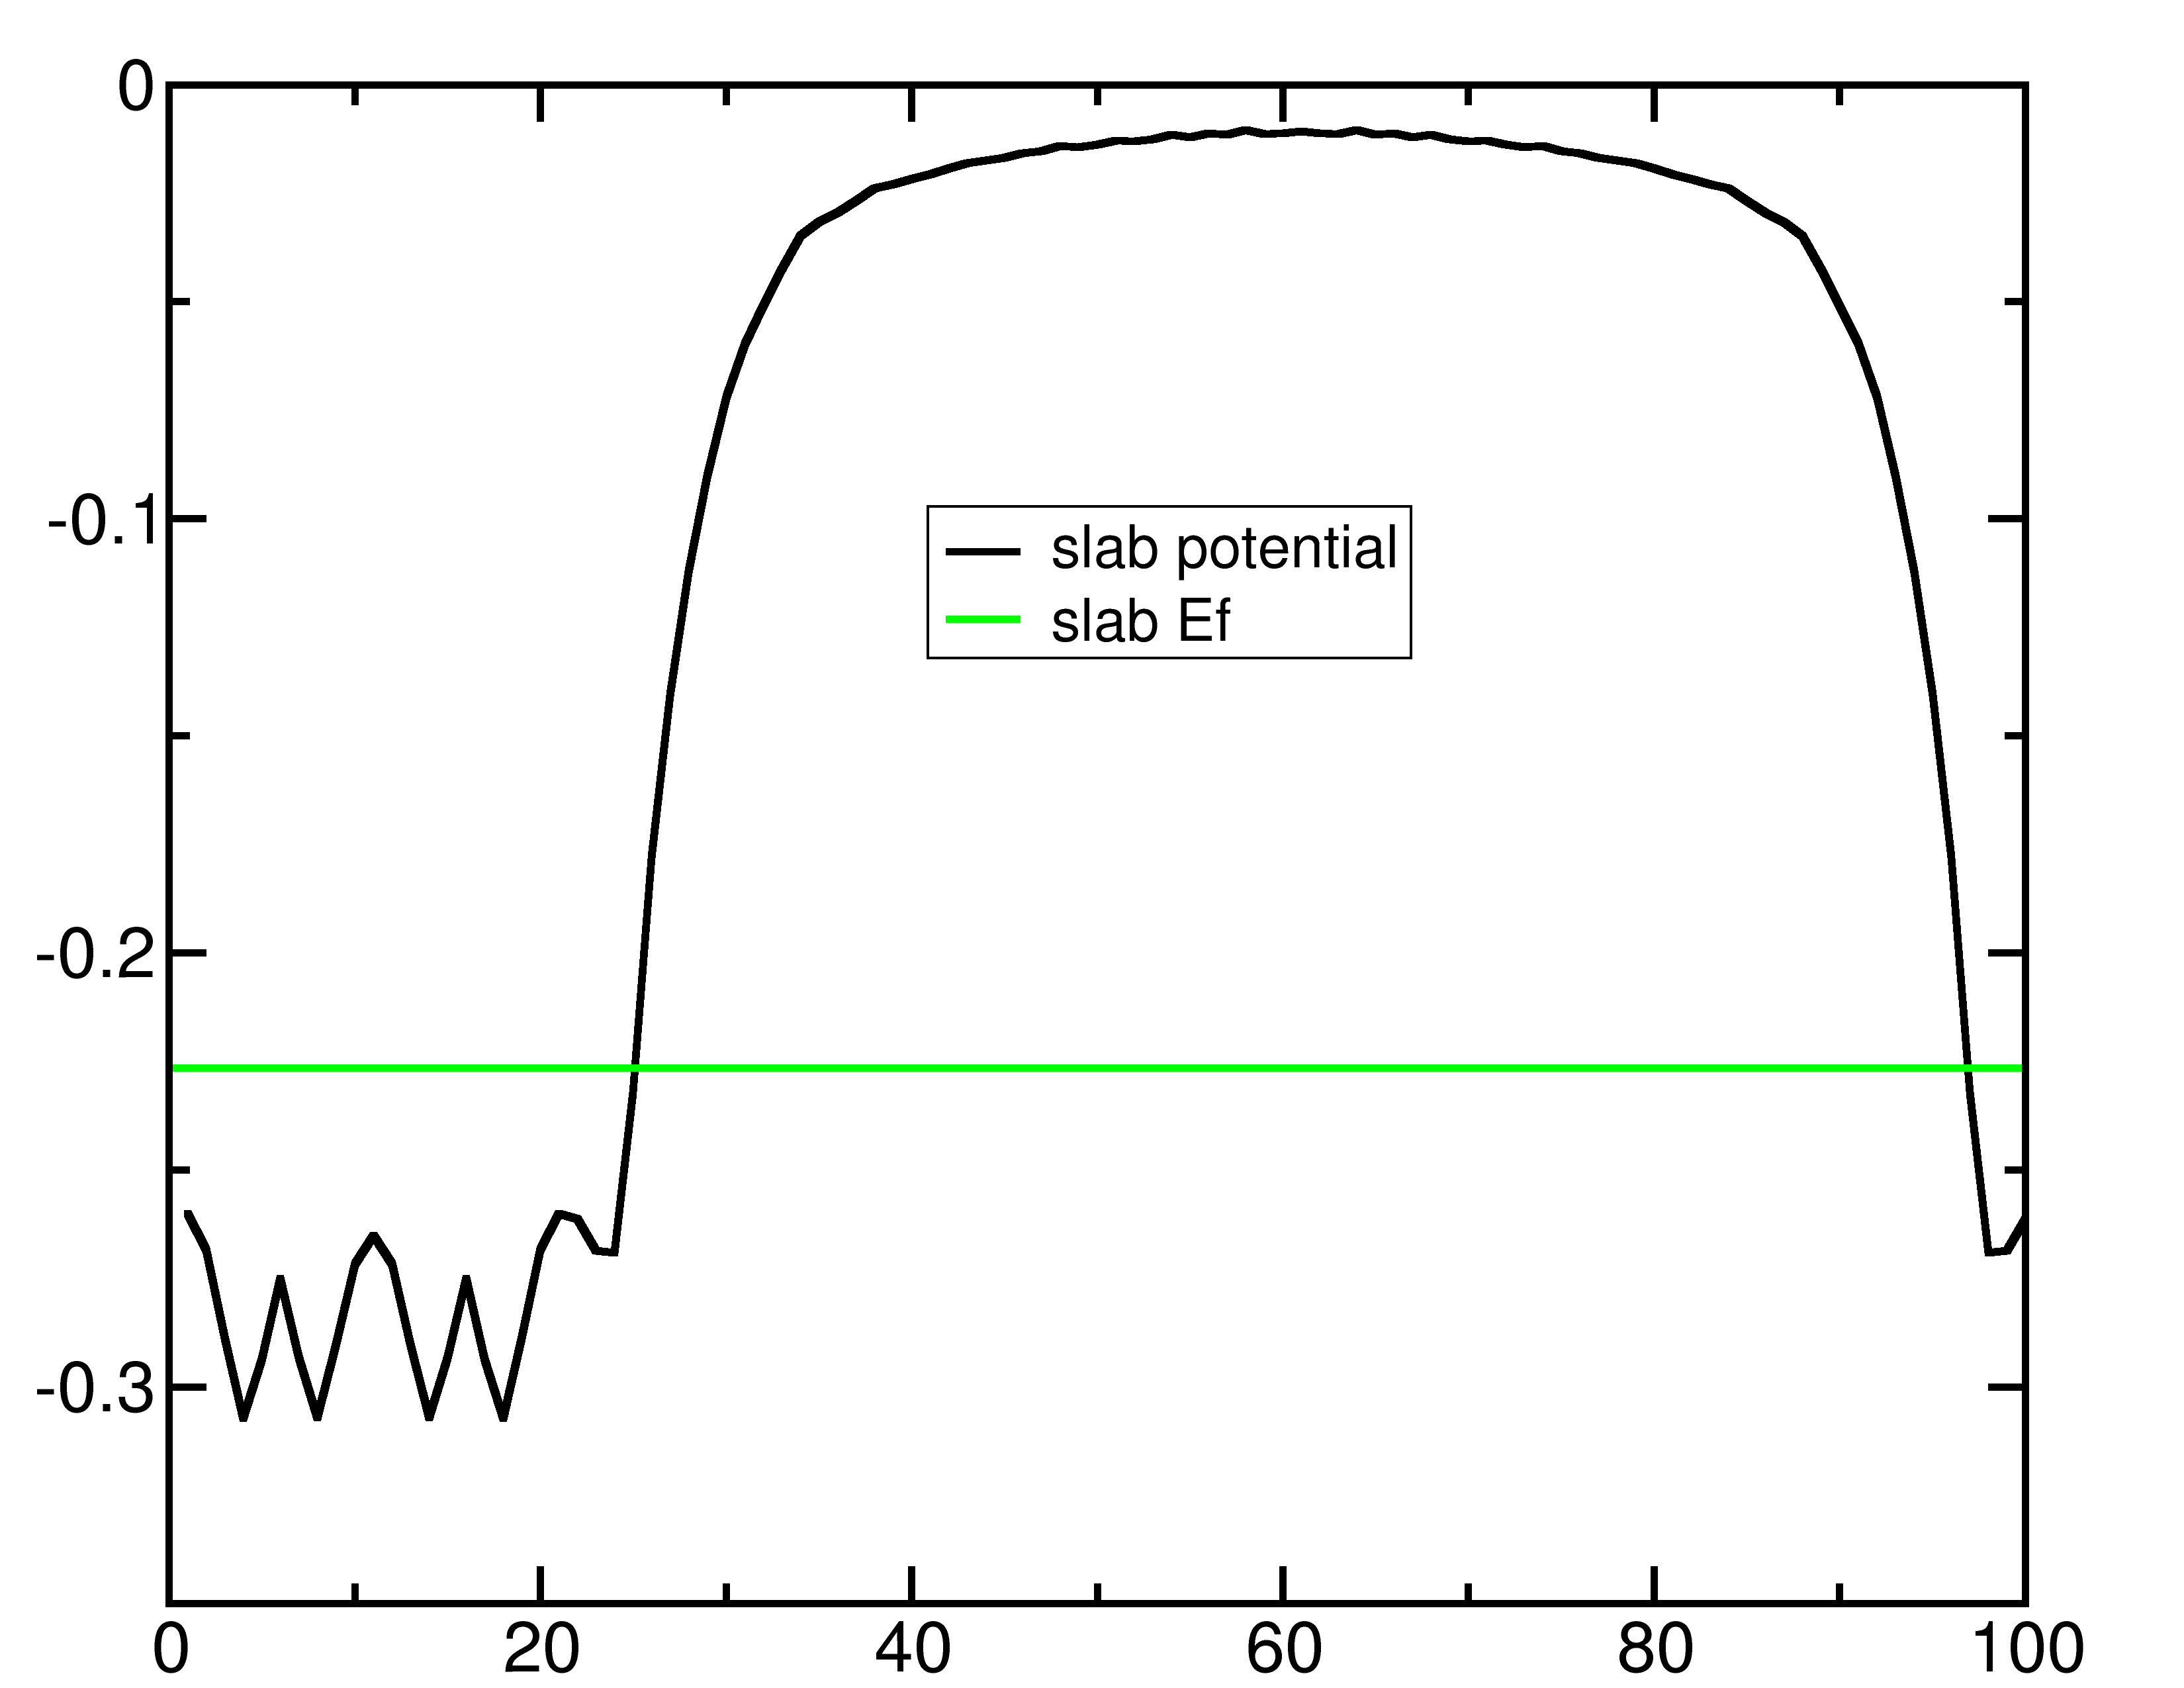
\includegraphics[width=0.8\linewidth]{workfunction_image0}
\caption{Potential and $E_F$ for a slab of 3 layers of (111) Gold}
\label{fig1}
\end{center}
\end{figure}

The important new input variable is \texttt{prt1dm} which triggers the output of the projected potential and density, along the 3 axes of the unit cell. These quantities are (in the case of the $z$ direction we are interested in):
\begin{eqnarray}
\bar{V}(z) &=& \int dx dy V(x,y,z) \\
\bar{\rho}(z) &=& \int dx dy \rho(x,y,z)
\end{eqnarray}
where $V$ is the electrostatic+xc (local) part of the potential (in Hartree), whereas $\rho$ is the electron density (in number of electrons / bohr$^3$).

Run the input file, using the pseudopotential 79au.pspnc - it should take less than a minute. The resulting output files are the usual ones (EIG, DEN, WFK) plus a new one, with a suffix 1DM, containing the projected density and potential. The file is ascii text, and organised into blocks, for projection on the first, then second, then third axis of the unit cell. The projection is along planes of points on the FFT grid - if your box is not orthogonal, the projection will not correspond to the cartesian projection! In our case the c axis is perpendicular to the other two, so we are fine. The first two columns of the file data contain the FFT index in the grid, and the fractional (reduced) coordinate of the plane for averaging. Then come the averaged potential, and the density. If you are a user of xmgrace or gnuplot, and have commented or chopped out the header and auxiliary information lines (this will be automatic from abinit v7.8), you can read in the data directly. The resulting plot for the z-projection is shown in Fig.~\ref{fig1}

You can see the potential goes up and has a plateau in the middle of the vacuum. One test of vacuum thickness convergence is that the plateau is indeed flat. Note that the potential does not go to 0 - the convention in abinit is that the electrostatic potential average over the \emph{whole} cell is 0, such that the vacuum part has to compensate the rest. Also shown is the Fermi energy of the slab, extracted from the output file. A first estimate of the work function is simply the difference between the potential plateau value and the Fermi level.

\section{Refinement of the Fermi level}
\begin{figure}[h]
\begin{center}
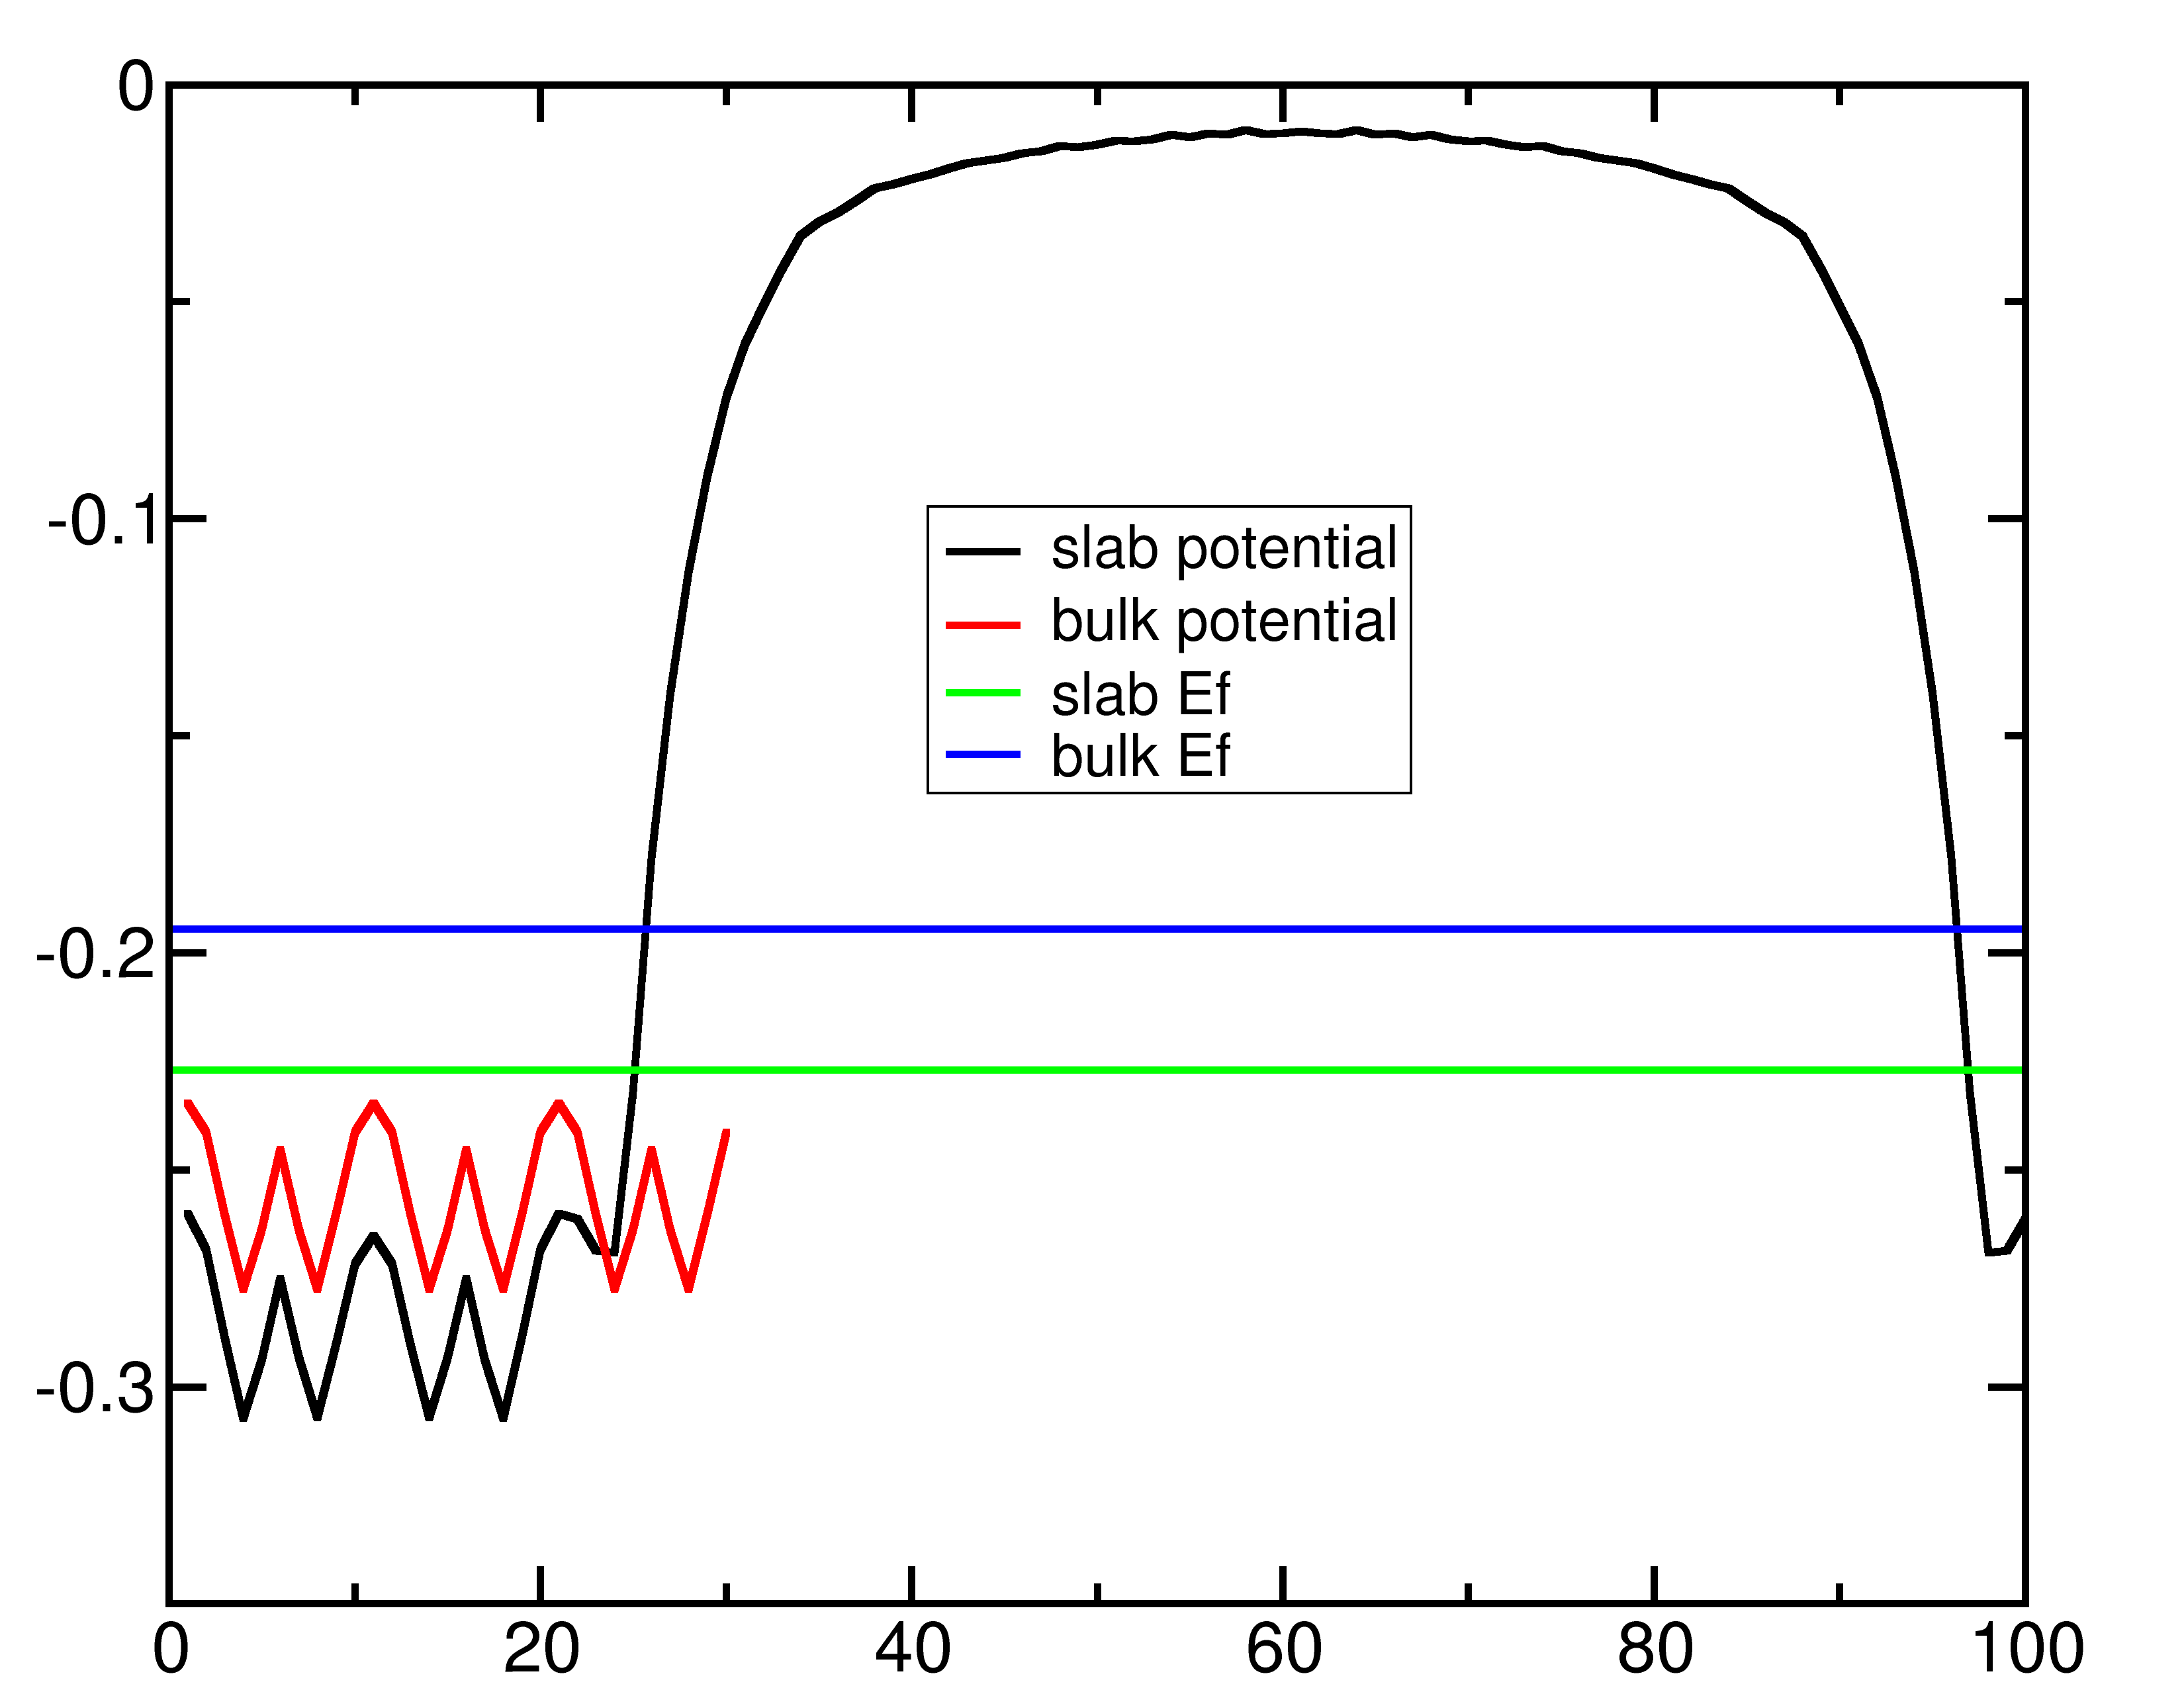
\includegraphics[width=0.48\linewidth]{workfunction_image1}
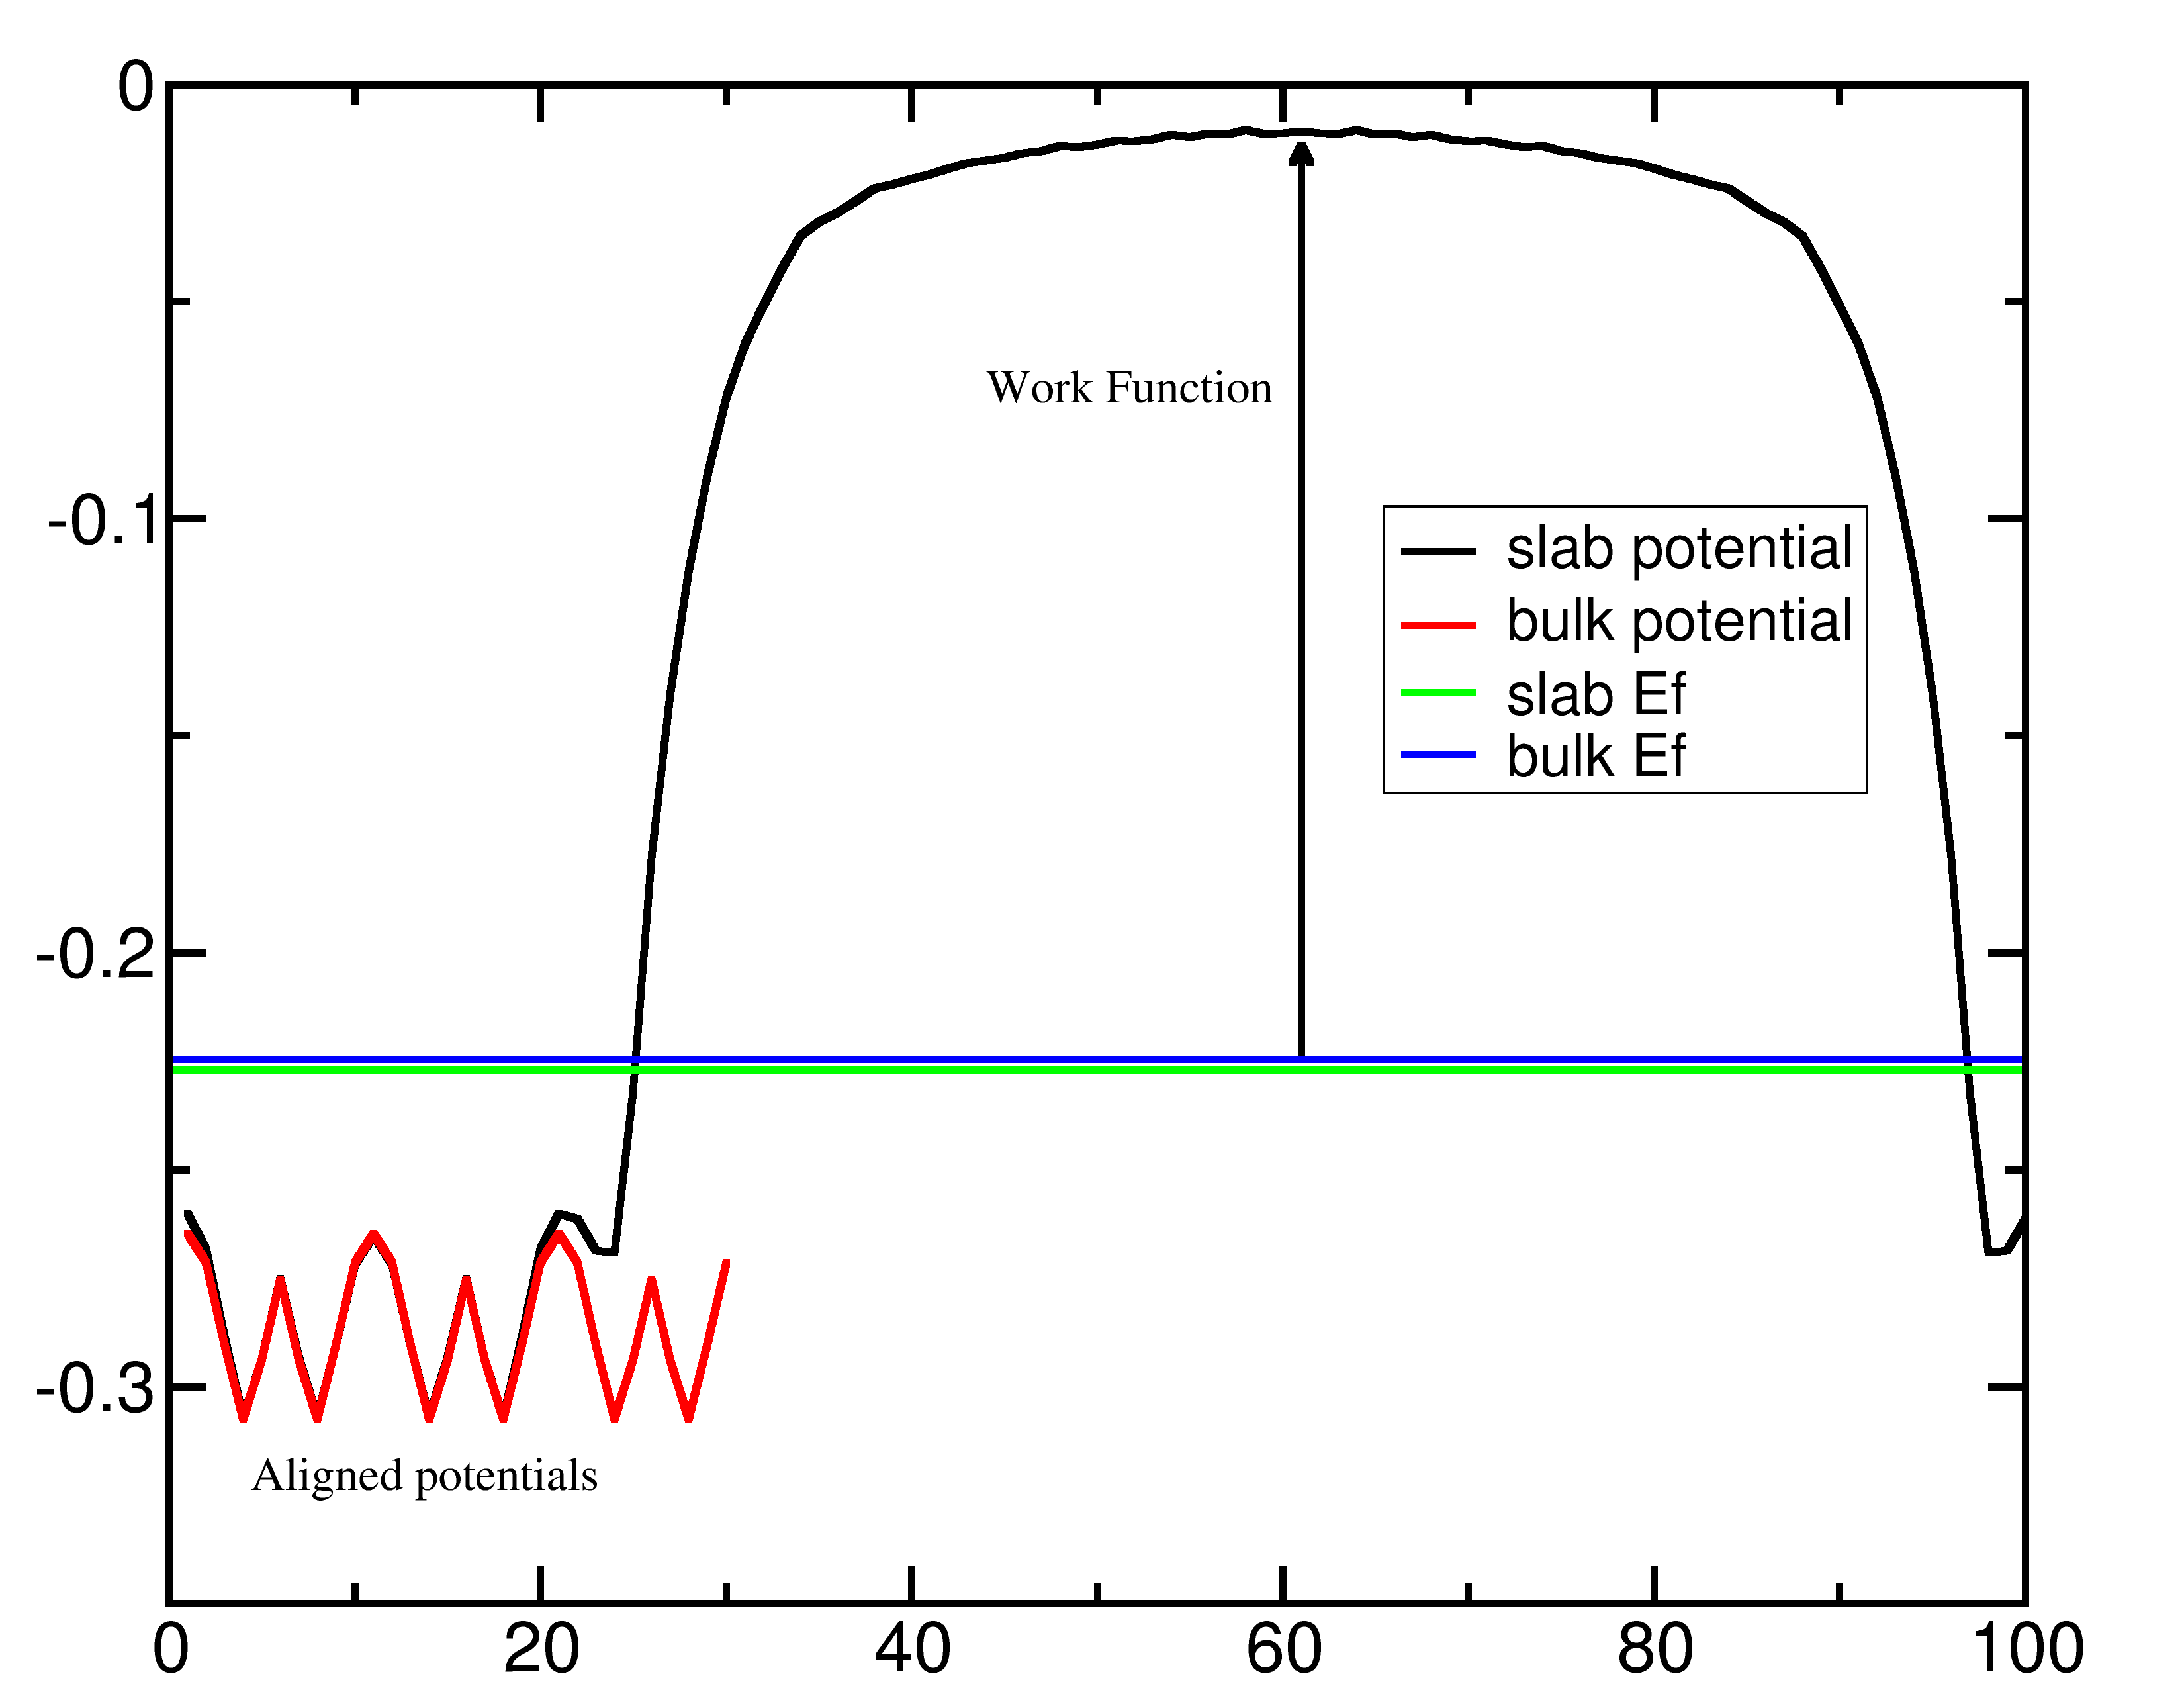
\includegraphics[width=0.48\linewidth]{workfunction_image2}
\caption{Potential and $E_F$ for a slab and a bulk, of 3 layers of (111) Gold. left: as produced by ABINIT; right: with the bulk quantities aligned to the potential in the center of the slab.}
\label{fig2}
\end{center}
\end{figure}

There is an additional correction which should be taken into account, due to the finite thickness of the slab. The total energy and surface relaxations can usually be converged with slabs of the order of 5-10 layers or a bit more (metals tend to screen well and converge a bit faster). However, if you consider the k-point sampling, this is equivalent to 5-10 k-points and is woefully insufficient in a metal. To compensate this we will do a supplementary correction of the position of $E_F$, taking it from a well converged continuous bulk calculation (with as many k-points as needed). To translate the bulk $E_F$ to the slab, we will need a common reference energy, which can not be the vacuum of course - there is none in the bulk. If your slab is thick enough, a local quantity we can compare is the potential, and it should be quite similar in the bulk and in the center of the slab.

You should now run the second input file, for the bulk system, and it should run even faster than the first. In principle you can use a primitive unit cell to get $E_F$, and this will also be the most efficient calculation. However, to get the planar averaged potential, you would need to do a little geometry and extract the real cartesian projection, which ABINIT does not do for you... For simplicity, we have replicated the same atoms as in the slab (same c direction) but removed the vacuum. As this cell is not primitive we set chkprim to 0 to force ABINIT to calculate it anyway. prt1dm is still turned on so we can get averaged $\bar{V}(z)$ to compare. The result is shown in Fig~\ref{fig2}(left): as you can see the potentials in the slab are very similar. If you shift the bulk potential and $E_F$ to align with the potential in the center of the slab (Fig~\ref{fig2}(right)) you can see a small difference in the $E_F$ values, which is the (quite small) correction for an infinitely thick slab.

The final result is shown in Fig~\ref{fig3}, converted to electron-volts. The resulting value is 5.82 eV, which is ridiculously close to the experimental 5.2 given how badly we are converged. This rough estimation often holds, as the work function for simple metals is mainly due to atomic properties and densities, but do not bet on it... In practical calculations, you do not necessarily need to plot things, but it is easier. Find the plateau value of $\bar{V}$ at position $z_1$, compare the potentials in bulk and slab inside the slab - position $z_0$ - (this is easier done graphically, but does not give you good numerical precision), and shift $E_F$ for the bulk by this difference, to get 
\begin{eqnarray}
\phi = \bar{V}_{slab}(z_1) - E_{F,bulk} - \bar{V}_{slab}(z_0) + \bar{V}_{bulk}(z_0)
\end{eqnarray}

\begin{figure}[h]
\begin{center}
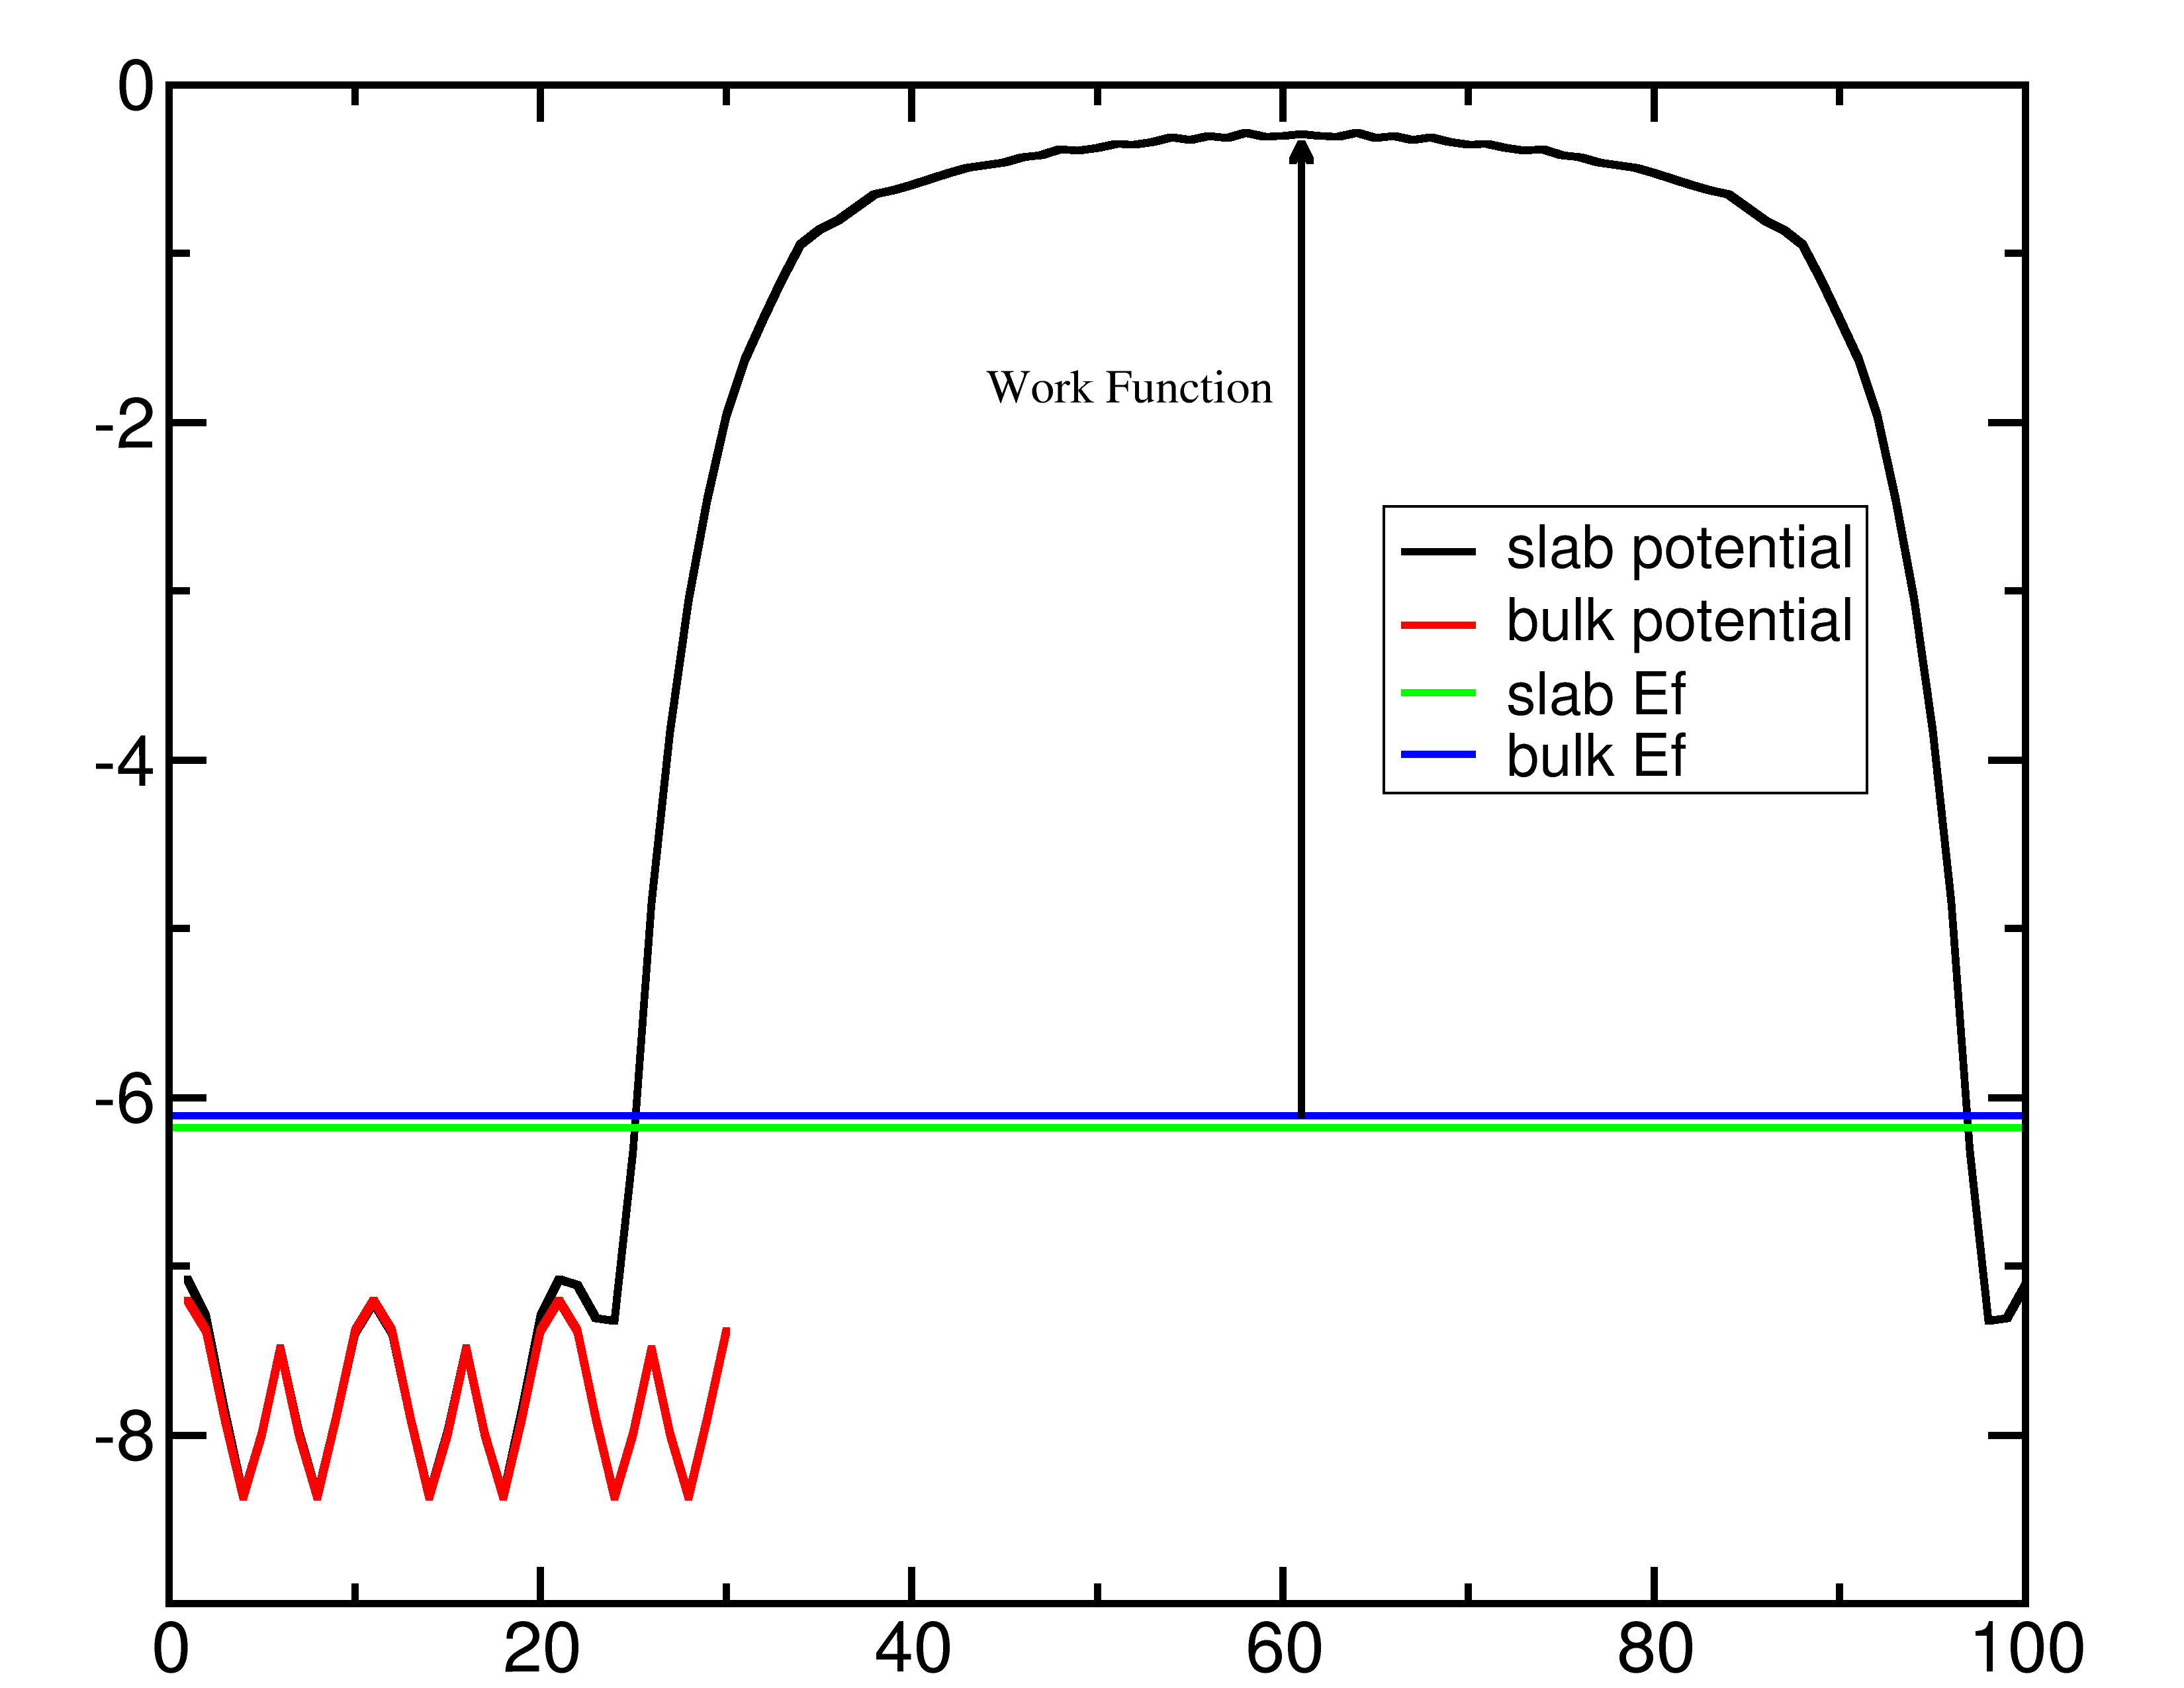
\includegraphics[width=0.8\linewidth]{workfunction_image3}
\caption{Potential and $E_F$ in eV for a slab and a bulk, of 3 layers of (111) Gold.}
\label{fig3}
\end{center}
\end{figure}

\section{Slab input file}
\begin{verbatim}
# bulk calculation for the z along 111 orientation of gold

prt1dm 1

ngkpt 4 4 1

# 4.07 cubic lattice parameter, 
# 5.76 in-plane 111 lattice parameter, and 
# 2.3498 interlayer distance -> 10 layers, 3 filled 7 vacuum
acell 2*5.76 23.498 Angstr
angdeg 90 90 120

ntypat 1
znucl 79
natom 3
typat 1 1 1

# z coordinate in tenths here!
xred
0 0 0
1/3 2/3 1/10
2/3 1/3 2/10

tolvrs 1.e-9

occopt 7
tsmear 0.0001

ecut 6
shiftk 0 0 0
\end{verbatim}

\section{Bulk input file}
\begin{verbatim}
# slab calculation for the 111 surface of gold

prt1dm 1
chkprim 0

ngkpt 4 4 4

# 4.07 cubic lattice parameter, 
# 5.76 in-plane 111 lattice parameter, and 
# 2.3498 interlayer distance -> 3 layers 0 vacuum
acell 2*5.76 7.0494 Angstr
angdeg 90 90 120

ntypat 1
znucl 79
natom 3
typat 1 1 1

# z coordinate in thirds here!
xred 
0 0 0
1/3 2/3 1/3
2/3 1/3 2/3

tolvrs 1.e-9

occopt 7
tsmear 0.0001

ecut 6
shiftk 0 0 0
\end{verbatim}


\end{document}
